\documentclass[a4paper,11pt]{report} \usepackage{anysize}
%\textwidth 6.0in \textheight = 664pt
\usepackage{xltxtra}
\usepackage{xunicode}
\usepackage{graphicx}
\usepackage{color}
\usepackage[table]{xcolor}
\usepackage{fancyvrb}
\usepackage{minted}
\usepackage{listings}
\usepackage{enumitem}
\usepackage{framed}
\usepackage{relsize}
\usepackage{float} 
\usepackage{fancyhdr}                                                          
\usepackage{lastpage}                                                          
\setmainfont[Mapping=TeX-text]{CMU Concrete}

\definecolor{bootred}{RGB}{248,148,6}
\definecolor{bootgreen}{RGB}{81,163,81}
\definecolor{bootblue}{RGB}{73, 178, 205}

% Finally, give us PDF bookmarks                                                   
\usepackage{color,hyperref}                                                        
\definecolor{darkblue}{rgb}{0.0,0.0,0.3}                                           
\hypersetup{colorlinks,breaklinks,                                                 
    linkcolor=darkblue,urlcolor=darkblue,                                          
    anchorcolor=darkblue,citecolor=darkblue}                                       

    % Layout: Puts the section titles on left side of page                         
    %\reversemarginpar                                                             
    %\setlength{\headheight}{15.2pt}                                                
    \pagestyle{plain}{ %                                                           
        \fancyhf{} % remove everything                                             
        \renewcommand{\headrulewidth}{0pt} % remove lines as well                  
        \renewcommand{\footrulewidth}{0.5pt}                                       
        \rhead{\leftmark}
        \rfoot{Page \thepage\ of \pageref{LastPage}}}
    \pagestyle{fancy}{ %                                                           
        \fancyhf{} % remove everything                                             
        \renewcommand{\headrulewidth}{0pt} % remove lines as well                  
        \renewcommand{\footrulewidth}{0.5pt}                                       
        \rhead{\leftmark}
        \rfoot{Page \thepage\ of \pageref{LastPage}}}


\begin{document}

\begin{titlepage}
\begin{center}
\begin{figure}[t] 
     
\includegraphics[scale=0.7]{title/ntua_logo}
\end{figure}
\begin{LARGE}\textbf{National Technical Univercity of Athens\\}\end{LARGE}
\begin{Large}
School of Electrical and Computer Engineering\\
\vspace{2cm}
Software Engineering\\
Software Design Document\\
Project Title: Spyglass\\
Academic Year 2012-2013\\
\end{Large}
\vspace{11cm}
\begin{tabular}{l r}
\Large{Alex Maurogiannis}&
\large{(03109677)}\\
\Large{Gregory Lyras}&
\large{(03109687)}\\
\end{tabular}\\

\vfill
\large\today\\
\end{center}
\end{titlepage}



\tableofcontents

\pagebreak

\large{Document Sign-Off}

\begin{table}[h]
    \begin{tabular}{| c | c | c | c |}
        \hline
        Name & R.N. & Signature & Date \\
        \hline
        Alex Maurogiannis & 03109677 & & \today \\
        \hline
        Gregory Lyras & 03109687 & & \today \\
        \hline
    \end{tabular}
\end{table}

\chapter{Introduction}
    \section{Purpose}
        The purpose of this document is to describe the design specifications
        of the \emph{spyglass} open source project.
    \section{Summary}
        This project aims to address the issue of dynamic content monitoring
        in a novel manner. Instead of searching on one site, we can monitor
        sites of interest and filter their updates based on keywords provided.
        If the updates match the search criteria then the end user is notified
        for the latest developments. The proposed project is a meta-search
        engine used to monitor sites for required information and provide
        notifications to its users accordingly. 
    \section{References}
        \begin{itemize}
                \item \href{https://www.djangoproject.com/}{django}
                \item \href{http://tastypieapi.org/}{tastypie}
                \item
                    \href{https://en.wikipedia.org/wiki/Representational_state_transfer}{REST framework}
                \item \href{https://github.com/mastergreg/spyglass-crawlie}{spyglass-crawlie}
                \item \href{https://github.com/afein/django-spyglass}{django-spyglass}
        \end{itemize}

\chapter{Design Choices}
    \section{Why Python}
        Python is a modern programming language. It features a dynamic type
        system and a strong object oriented model. It emphasises on code
        readability and less lines of code. One of its strongest features is
        'batteries included' and easy interfacing with C libraries. This
        provides a large ecosystem of available modules and libraries to
        choose from. When facing the task of such complexity as a generic web
        application, a programming language with the above features seems a
        good choice.
    \section{Why Django}
        The \emph{django} framework is a highly extensible modern web
        framework with a plethora of ready-to-use capabilities such as
        object-relation modelling, session management, dynamic templating and
        multiple \emph{DBMS} support that simplify the development of web
        applications. Instead of developing a web application from scratch we
        decided to utilise \emph{django's} features to focus on the task at
        hand.
    \section{Why REST}
        Given the recent advances in the standardisation of web Application
        Programming Interfaces (APIs) the use of RESTful architectural methods
        is highly preferable in contradiction to deprecated remote procedure
        call architectures such as SOAP. Additionally, there are several
        modules that allow django to provide RESTful APIs.
    \section{Crawler Network}
        The main design concept behind this project is to provide realtime
        monitoring of multiple resources. In order to provide this feature we
        designed a distributed method of crawling that provides the network
        with resilience against blocking. Thus we distribute the set of
        crawlers on several machines that operate independently and
        concurrently.
    \section{Crawler Protocol}
        The protocol used by the crawlers when they interact with the server
        provides the following operations. 
        \begin{itemize}
                \item \emph{Get Sites}: The crawler requests through HTTP a
                    list of websites supported by the server.
                \item \emph{Get XPaths}: The crawler requests through HTTP the
                    XPaths for every field of interest for each crawlable
                    website.
                \item \emph{Get Workload}: The crawler requests through HTTP a
                    list of queries to be resolved.
                \item \emph{Send Result}: If a query is resolved the crawler
                    sends through HTTP the data back to the server.
                \item \emph{Update Timestamps}: When the query is not resolved
                    the crawler sends a PATCH request to the server regarding
                    the unresolved query in order to update the query's
                    timestamp.
        \end{itemize}

\chapter{System Architecture}
    \begin{figure}[h]
        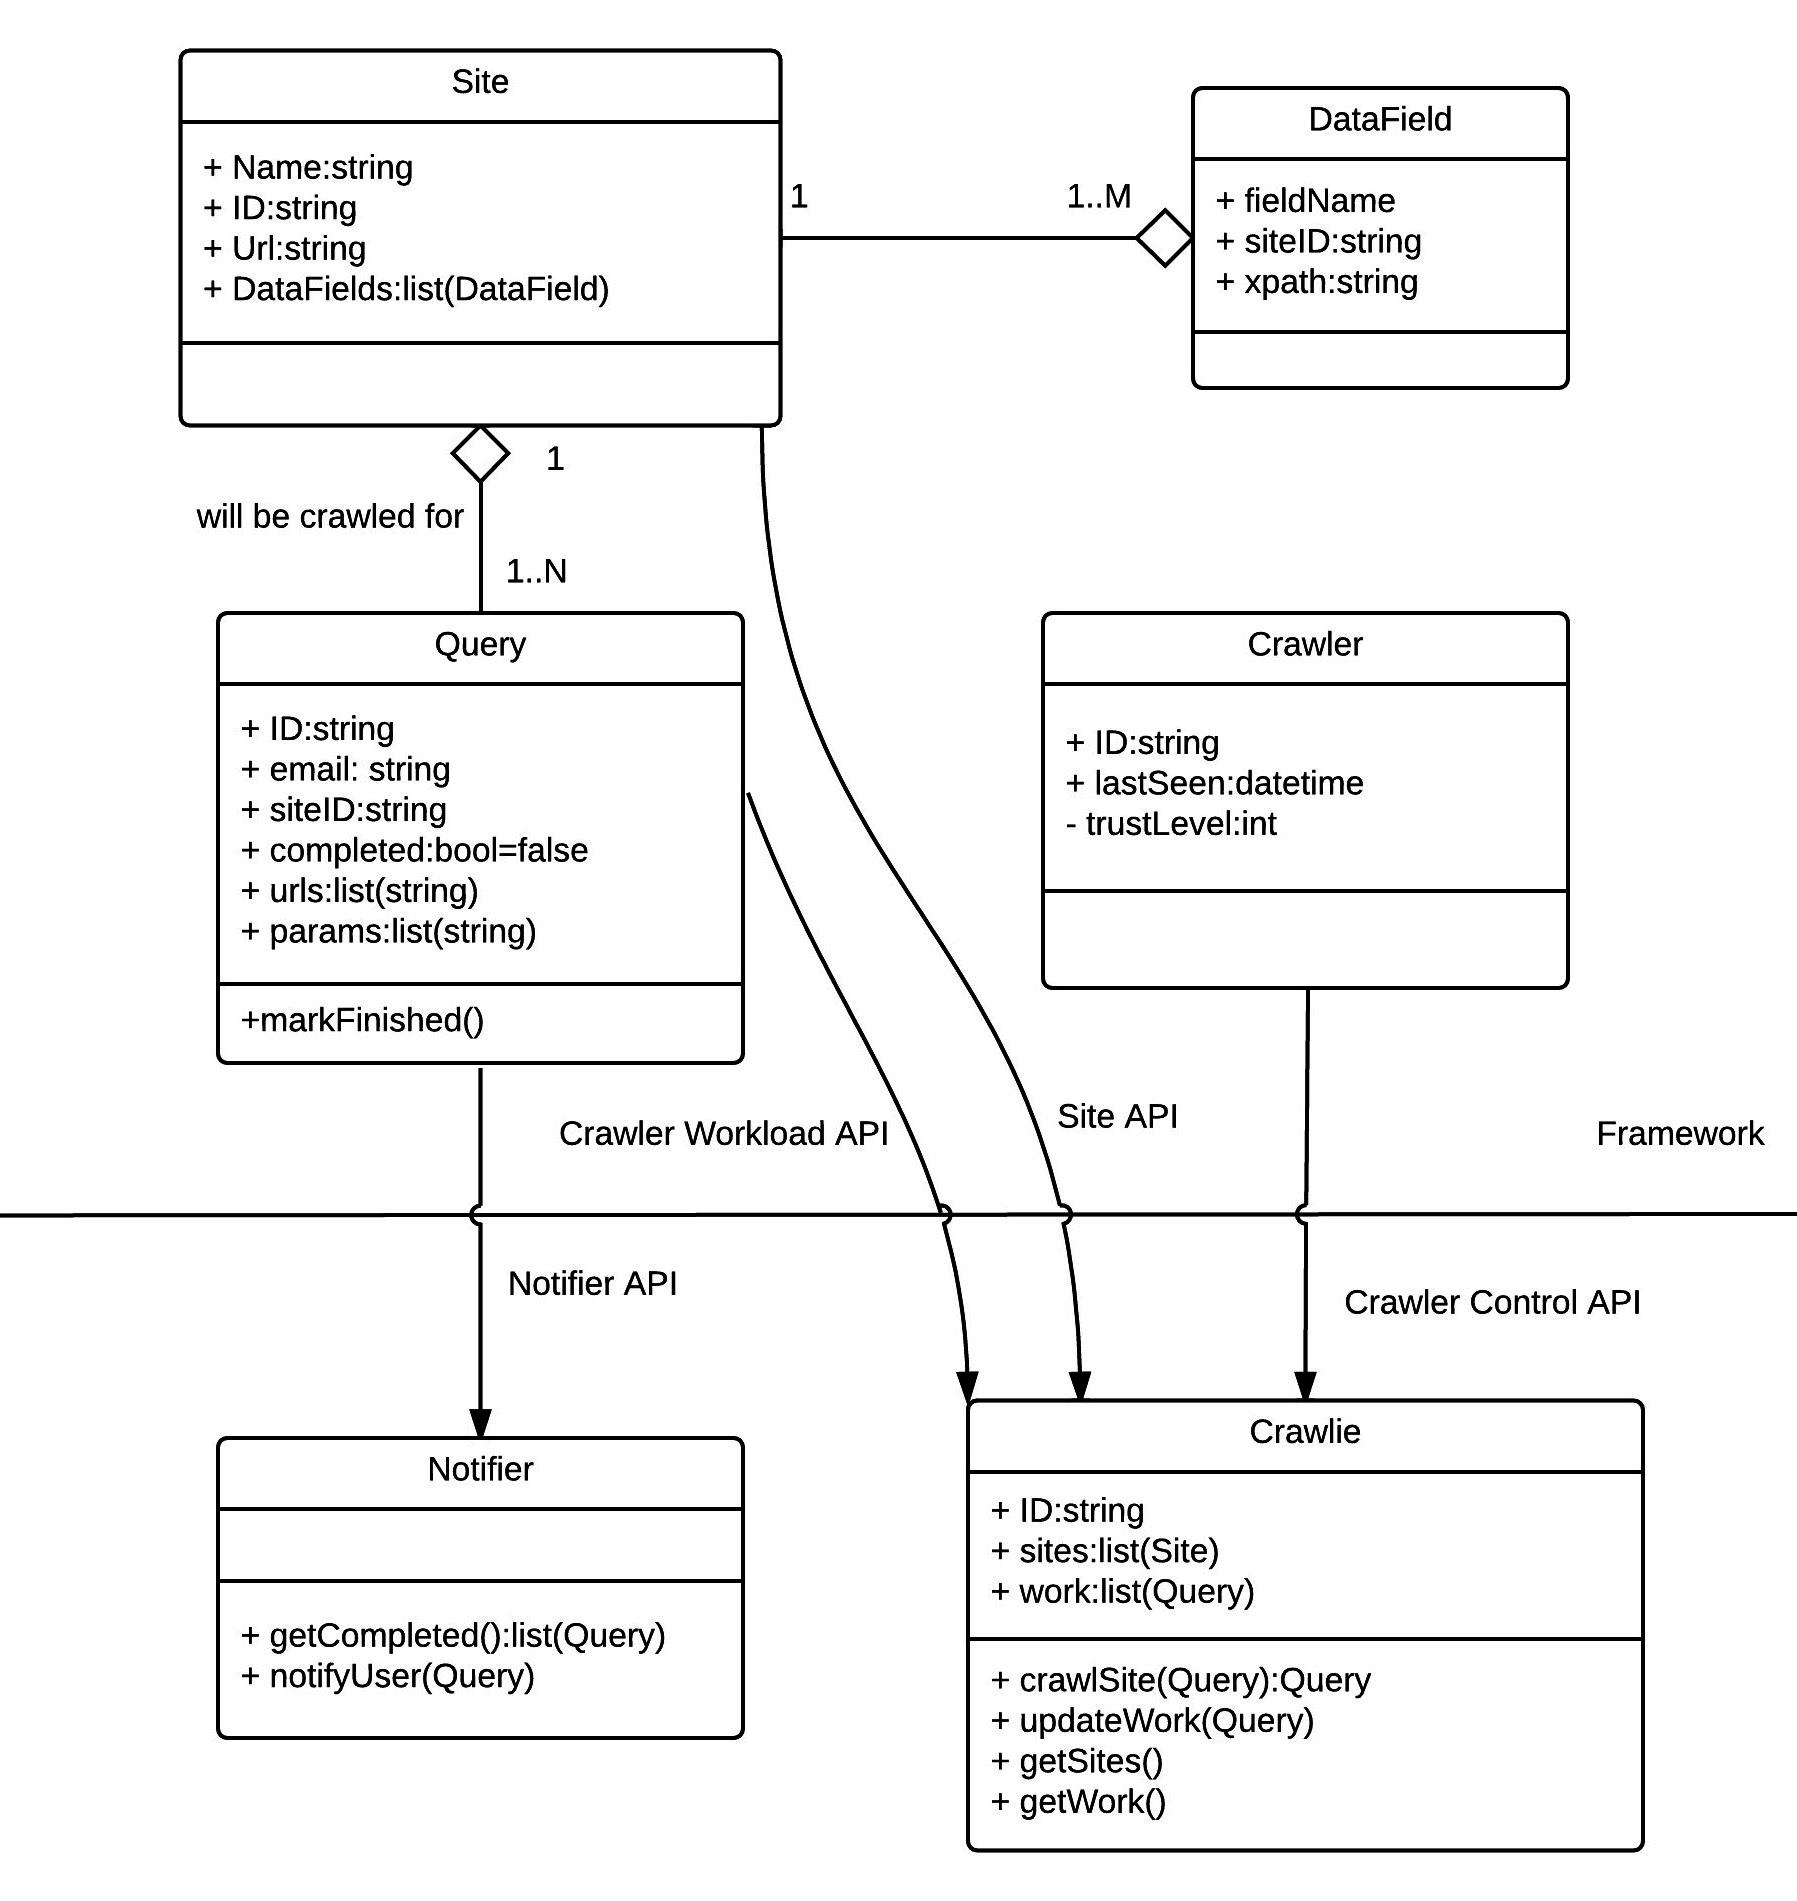
\includegraphics[width=\textwidth]{files/high_level_diagram.png}
        \caption{Draft Class Diagram}
        \label{fig:high_level_diagram}
    \end{figure}

    \begin{figure}[h]
        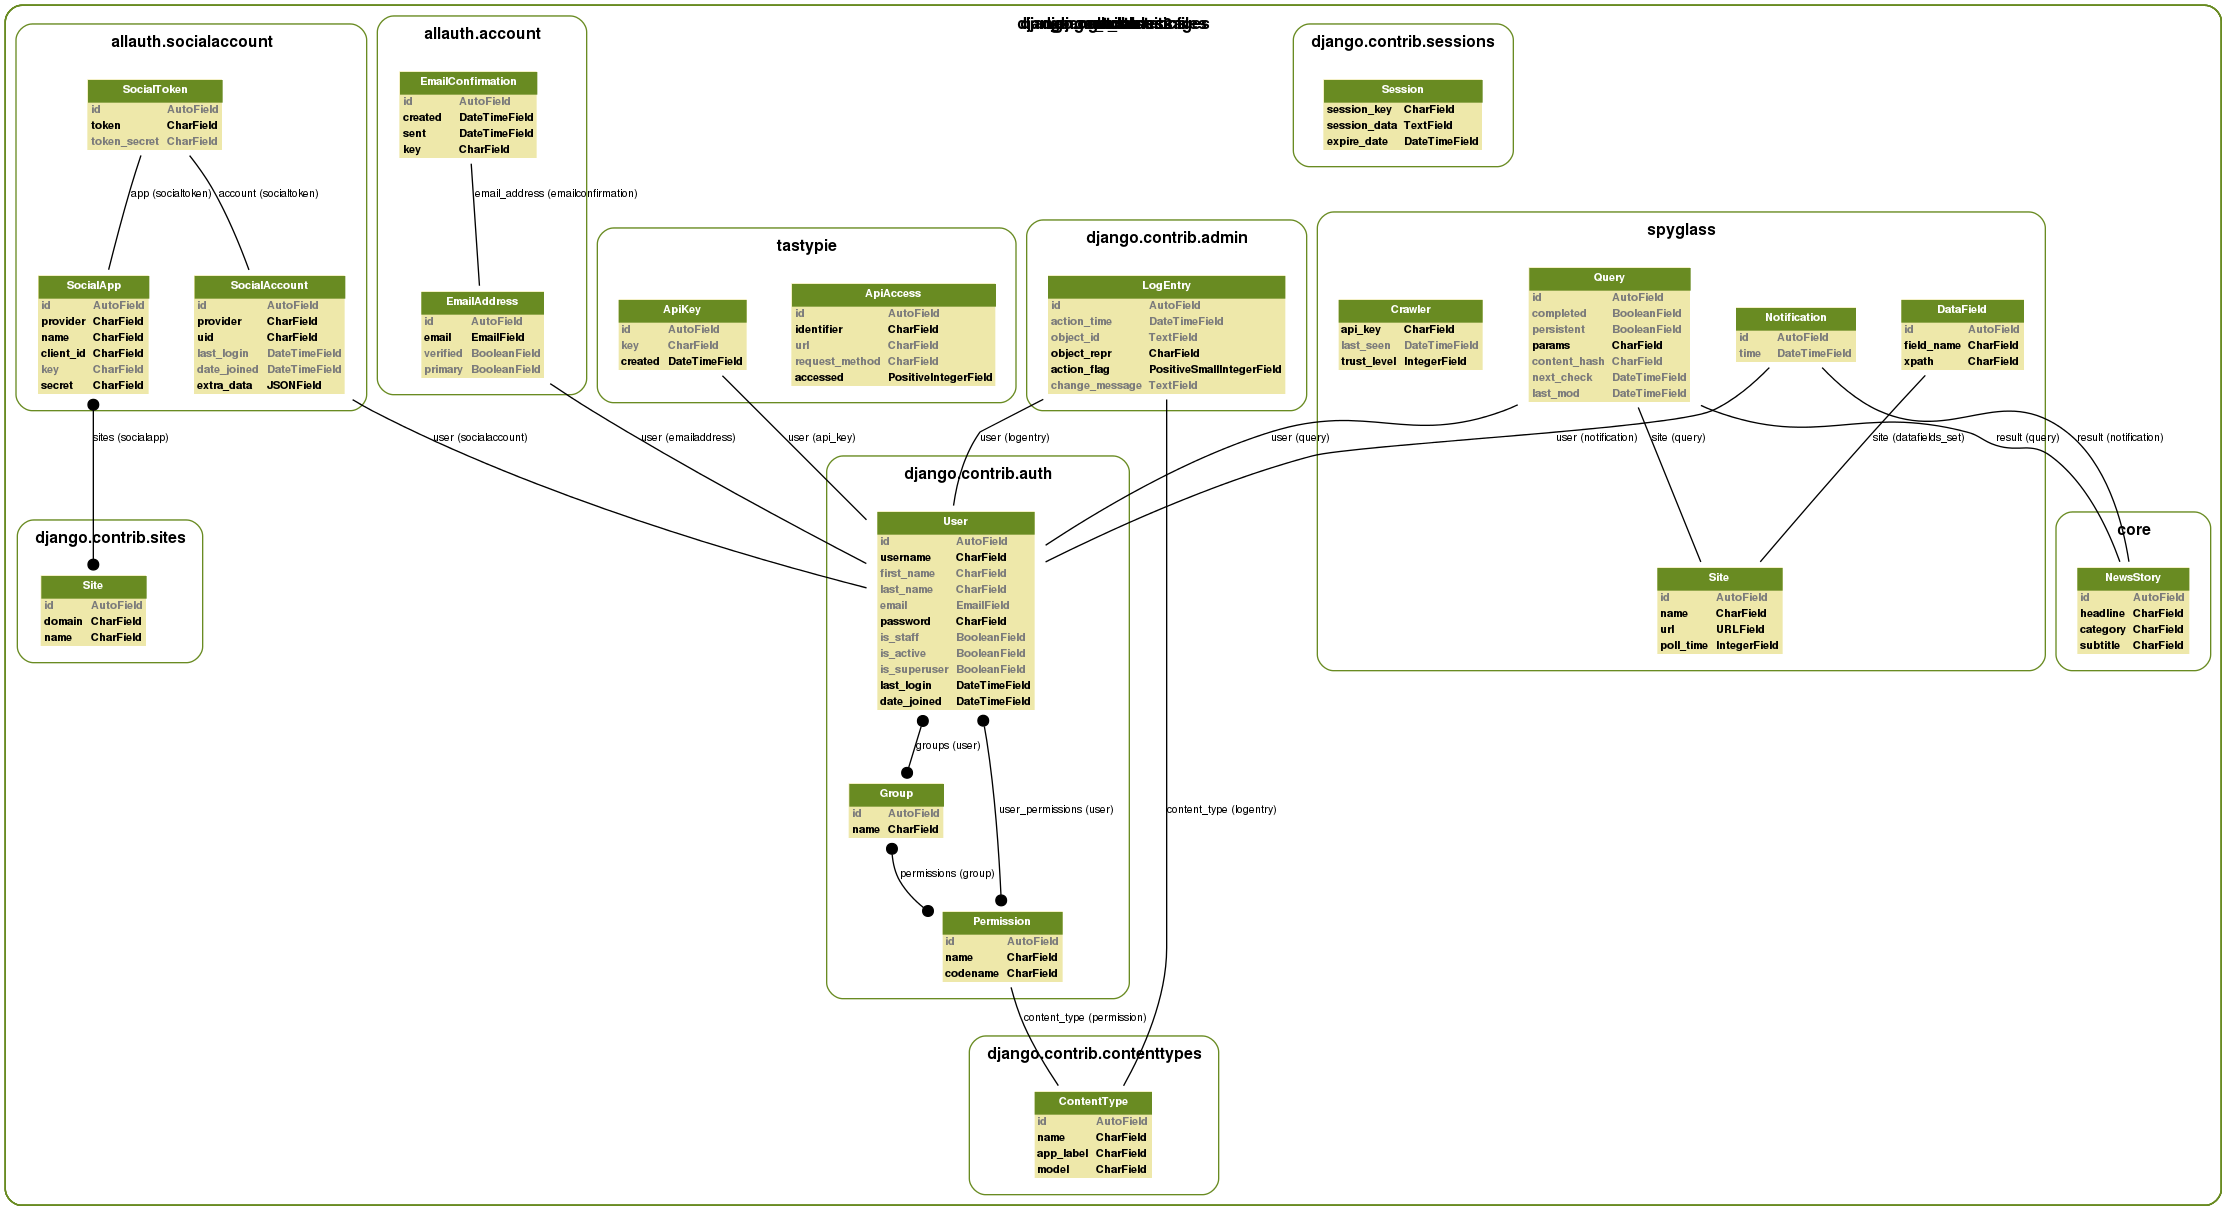
\includegraphics[angle=90,height=\textheight]{files/spyglass.png}
        \caption{Component Diagram}
    \end{figure}

\chapter{Class Details}
    \section{REST APIs}
    \inputminted[linenos,fontsize=\scriptsize,frame=leftline]{text}{files/api}
    \section{Crawlie}
    \inputminted[linenos,fontsize=\scriptsize,frame=leftline]{text}{files/crawlie}
    \section{Models}
    \inputminted[linenos,fontsize=\scriptsize,frame=leftline]{text}{files/models}
    \section{Views}
    \inputminted[linenos,fontsize=\scriptsize,frame=leftline]{text}{files/views}
    \section{Unittests}
    \inputminted[linenos,fontsize=\scriptsize,frame=leftline]{text}{files/unittests}
    \section{Misc}
    \inputminted[linenos,fontsize=\scriptsize,frame=leftline]{text}{files/tags}

\chapter{State Diagrams}

\chapter{Open Subjects}
    \section{Improved Searching}
        Right now the crawlers target only text and use text similarity
        routines to determine a ratio. This ratio signifies how relative are
        the user provided query terms to the content currently found in the
        webpages. In the future it is possible to unify the searching process
        and provide smarter matches that focus on conceptual matching instead
        of text.
    \section{Network of trust in crawlers}
        In the current implementation the crawlers are considered trustworthy.
        This provides the crawlers with infinite power over the unfinished
        database query entries. The above approach can be extended to provide
        a point system over each crawlers API key, by verifying the result
        using multiple crawlers over a single query.
    \section{Centralised configuration for crawlers}
        At the moment each crawler has a local configuration for server
        polling intervals. This can be a security issue for a large number of
        crawlers. The system should be able to balance the load with the use
        of a configuration mechanism handled through another API.
\end{document}
